\begin{figure}[!htbp]
\centering
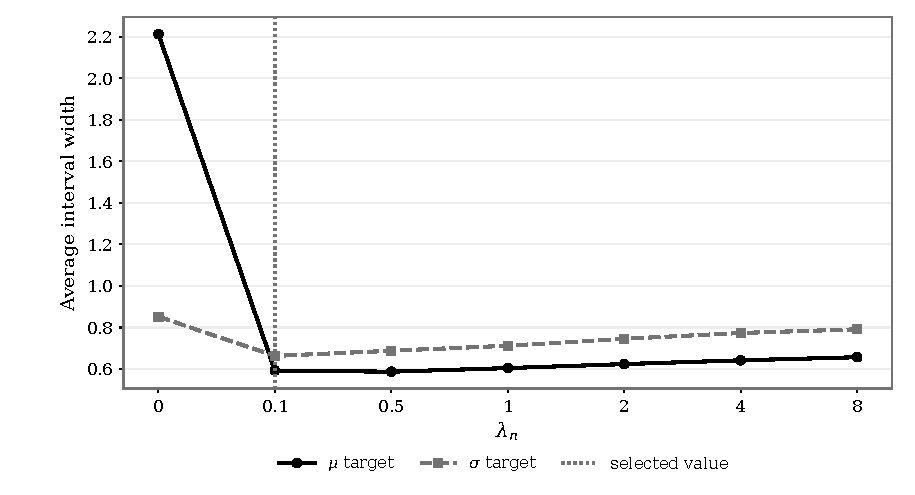
\includegraphics[width=0.78\linewidth]{results/figures/fig_lambda_sensitivity.pdf}
\caption{Sensitivity to the penalty weight $\lambda_n$: average interval width for each target, $1000$ replications per grid point. Grid points are drawn at equal spacing because the design grid is geometric. The $\mu$-target width falls from $2.213$ at $\lambda_n=0$ to $0.593$ at the selected value $\lambda_n=0.1$ and then rises slowly, so the penalty is not a technical convenience: with no Mahalanobis term the comparison rests on a single linear projection and the profile objective is nearly flat in the nuisance direction. Coverage clears the Monte-Carlo-adjusted floor $0.9365$ at every grid point, so the figure concerns width alone. This sweep locates endpoints to a coarser bisection tolerance than Table~\ref{tab:exp1-main}, so its absolute widths are not comparable with that table although the ordering in $\lambda_n$ is unaffected.}
\label{fig:lambda-sensitivity}
\end{figure}
